% -------------------------------------------------------------------------
% Setup
% -------------------------------------------------------------------------
\documentclass[11pt, aspectratio=149]{beamer}
% Options for aspectratio: 1610, 149, 54, 43 and 32, 169
\usepackage[utf8]{inputenc}
\usepackage[english]{babel}% Alternative: 'norsk'
\usepackage[expansion=false]{microtype}% Fixes to make typography better
\usecolortheme{beaver} % Decent options: beaver, rose, crane
\usepackage{booktabs}% Professional tables

% Turn off on on default math font
\usepackage{mathptmx}


\title{Speed dates with optimization problems}
\subtitle{10 problems in 10 minutes}
\institute{}
\author{{\footnotesize tommyod @ GitHub}}
\date{February 15, 2019}

% -------------------------------------------------------------------------
% Package imports
% -------------------------------------------------------------------------
\usepackage{etoolbox}
\usepackage{graphicx}
\usepackage{amsmath}
\usepackage{amsfonts}
\usepackage{amssymb}
\usepackage{mathtools}
\usepackage{graphicx}
\usepackage{hyperref}
\usepackage[sharp]{easylist}
\usepackage{multicol}

\usefonttheme{professionalfonts}
\usepackage{fontspec}
\setmainfont{Open Sans}
\setsansfont{Open Sans}
\setmonofont{Ubuntu Mono}
\usefonttheme{serif}

% https://tex.stackexchange.com/questions/115223/how-insert-male-and-female-symbol
\usepackage{wasysym}

\usepackage{blkarray} %https://tex.stackexchange.com/questions/59517/label-rows-of-a-matrix-by-characters

%gets rid of bottom navigation bars
\setbeamertemplate{footline}[frame number]{}

%gets rid of bottom navigation symbols
\setbeamertemplate{navigation symbols}{}

% Set up colors to be used
\definecolor{purered}{RGB}{31,119,180}
\definecolor{titlered}{RGB}{31,119,180}
\definecolor{bggray}{RGB}{242,242,242}
\definecolor{bggraydark}{RGB}{217,217,217}

% Change the default colors

\setbeamercolor*{title}{bg=bggray,fg=titlered}
\AtBeginEnvironment{theorem}{%
	\setbeamercolor{block title}{fg=titlered, bg=bggraydark}
	\setbeamercolor{block body}{fg=black,bg=bggray}
}
\AtBeginEnvironment{proof}{%
	\setbeamercolor{block title}{bg=bggraydark}
	\setbeamercolor{block body}{fg=black,bg=bggray}
}
\AtBeginEnvironment{example}{%
	\setbeamercolor{block title example}{bg=bggraydark}
	\setbeamercolor{block body example}{fg=black,bg=bggray}
}
\AtBeginEnvironment{definition}{%
	\setbeamercolor{block title}{bg=bggraydark}
	\setbeamercolor{block body}{fg=black,bg=bggray}
}

\setbeamercolor{block title example}{bg=bggraydark}
\setbeamercolor{block body example}{fg=black,bg=bggray}
\setbeamercolor{block title}{bg=bggraydark}
\setbeamercolor{block body}{fg=black,bg=bggray}

\setbeamercolor{frametitle}{fg=titlered,bg=bggray}
\setbeamercolor{section in head/foot}{bg=black}
\setbeamercolor{author in head/foot}{bg=black}
\setbeamercolor{date in head/foot}{fg=titlered}


% Spacing for lists
\newcommand{\listSpace}{0.4em}

% Theorems, equations, definitions setup
\theoremstyle{plain}

\makeatletter
\patchcmd{\beamer@sectionintoc}
{\vfill}
{\vskip\itemsep}
{}
{}
\makeatother  

\AtBeginSection[]{
	\begin{frame}
		\vfill
		\centering
		\begin{beamercolorbox}[sep=8pt,center,shadow=false,rounded=false]{title}
			\usebeamerfont{title}\insertsectionhead\par%
		\end{beamercolorbox}
		\vfill
	\end{frame}
}

\newcommand{\norm}[1]{\left\lVert#1\right\rVert}

% -------------------------------------------------------------------------
% Document start
% -------------------------------------------------------------------------
\begin{document}
\maketitle
	
% -------------------------------------------------------------------------
\begin{frame}[fragile]{Introduction}
	
	\begin{equation*}
	\text{Understand}
	 \, \leftrightarrow \,
	 \textbf{Search} 
	 \, \leftrightarrow \,
	 \text{Solve}
	\end{equation*}
	
	\begin{columns}
		\begin{column}{0.55\textwidth}
	\begin{easylist}[itemize]
		\ListProperties(Space=\listSpace, Space*=\listSpace)
		# Efficient algorithms exist for many problems.
		# Implementations of these algorithms are also available.
		# The remaining difficulty is often having enough prior knowledge to recognize a problem. 
	\end{easylist}
		\end{column}
		\begin{column}{0.45\textwidth}%
			\begin{figure}
				\centering
				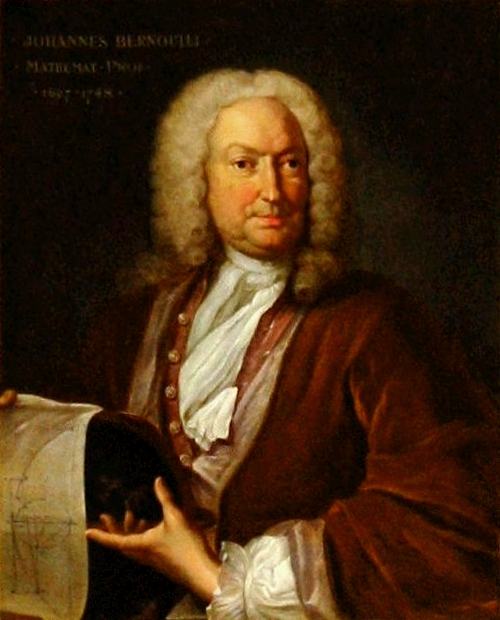
\includegraphics[width=0.75\linewidth]{figs/Johann_Bernoulli.jpg}
				\caption{{\scriptsize Johann Bernoulli, circa 1740}}
			\end{figure}
		\end{column}
	\end{columns}
\end{frame}

% -----------------------------------------------------------------------------

\begin{frame}[fragile, t]{(1) The paper box problem}
\begin{columns}
\begin{column}{0.55\textwidth}
\textbf{Introduction}\\ \vspace*{0.5em} 
Given a square piece of paper, cut the paper at a location $x$ to maximize the volume of the resulting box. \\
\vspace*{1em}
This problem can be formulated as
\begin{align*}
\text{minimize } \quad & -V(x, s) = -s^2 x  \\
\text{subject to } \quad & 2x + s = L \\
& s, x \geq 0.
\end{align*}
\end{column}
\begin{column}{0.45\textwidth}%
	\begin{figure}
		\centering
		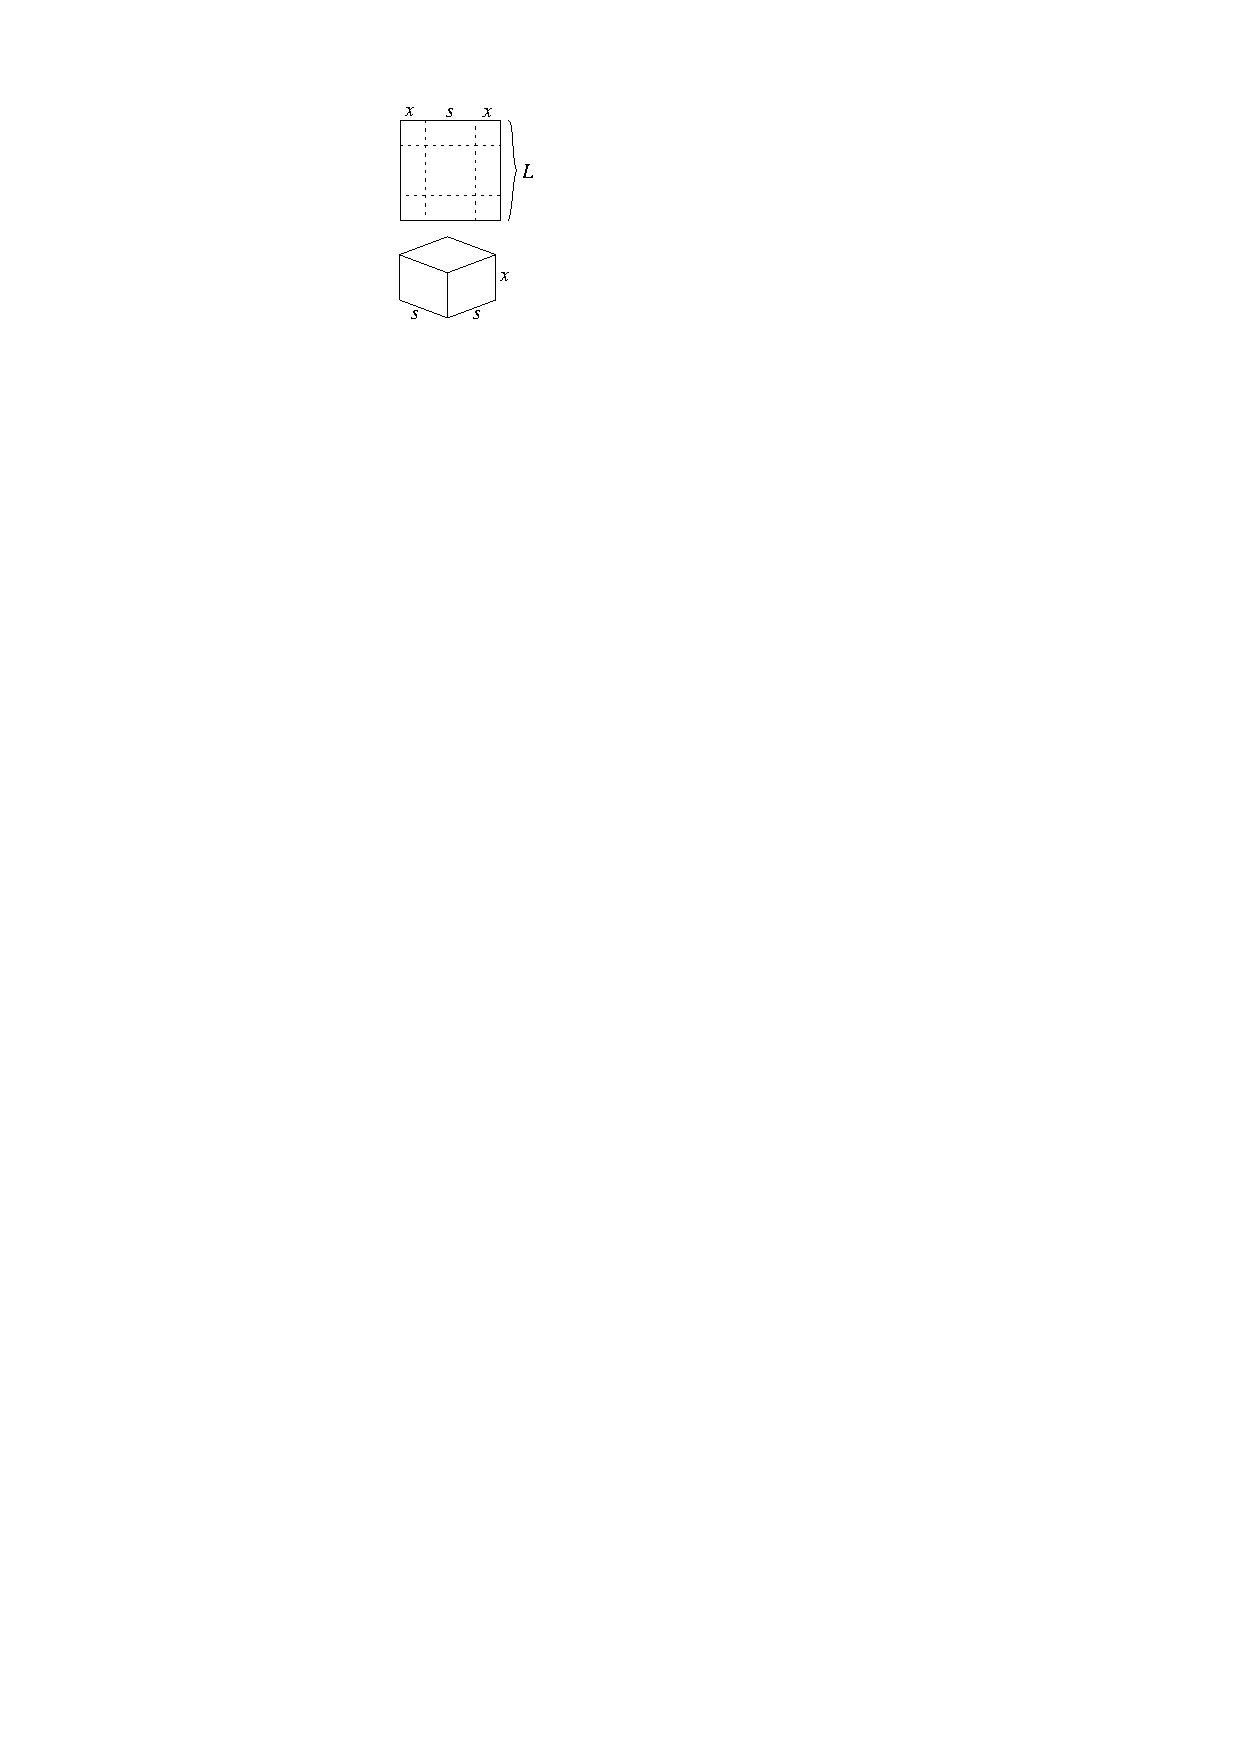
\includegraphics[width=0.75\linewidth]{figs/box_opt.pdf}
	\end{figure}
\end{column}
\end{columns}
\end{frame}


\begin{frame}[fragile, t]{(1) The paper box problem}
\begin{columns}
\begin{column}{0.55\textwidth}
\textbf{Problem instance}
\begin{align*}
\text{minimize } \quad & -V(x) = -(L - 2x)^2 x  \\
\text{subject to } \quad & x \geq 0 \\
& x \leq L/2
\end{align*}
\textbf{Problem generalization}
\\
\vspace*{0.5em} 
Given a smooth function $f: \mathbb{R} \to \mathbb{R}$.
\begin{align*}
	\text{minimize } \quad & f(x) \\
	\text{subject to } \quad & x \geq a \\
	 & x \leq b
\end{align*}
Solved using differentiation.
\end{column}
\begin{column}{0.45\textwidth}%
	\begin{figure}
		\centering
		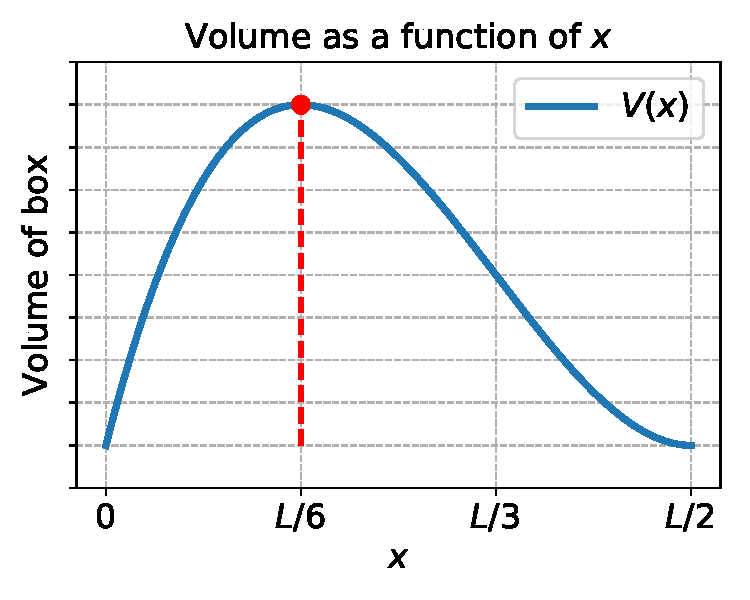
\includegraphics[width=1.05\linewidth]{figs/paper_box_volume.pdf}
	\end{figure}
\end{column}
\end{columns}
\end{frame}

% -----------------------------------------------------------------------------

\begin{frame}[fragile, t]{(2) The industrial box problem}
	\begin{columns}
		\begin{column}{0.6\textwidth}
			\textbf{Introduction}\\ \vspace*{0.5em} 
			Given a square meter price for the material of a box with no lid, construct the cheapest box having unit volume.\\
			\vspace*{1em}
			This problem may be formulated as
			\begin{align*}
			\text{minimize } \quad & P(x, y, x) = xy + 2yz + 2xz  \\
			\text{subject to } \quad & V(x, y, z) = xyz = 1 \\
			& x, y, z \geq 0.
			\end{align*}
		\end{column}
		\begin{column}{0.4\textwidth}%
		\begin{figure}
			\centering
			
\includegraphics[width=1.05\linewidth]{figs/box_opt_lagrange.pdf}
		\end{figure}
		\end{column}
	\end{columns}
\end{frame}


\begin{frame}[fragile, t]{(2) The industrial box problem}
	\begin{columns}
		\begin{column}{0.6\textwidth}
			\textbf{Problem instance} \\
			Construct a \emph{Lagrange function} $L(x, y, z, \lambda)$, solve the equations
			\begin{alignat*}{3}
			L_x &= y + 2z + \lambda yz &&= 0 \\
			L_y &=x + 2z + \lambda xz &&= 0 \\
			L_z &=2 (x + y) + \lambda xy &&= 0 \\
			L_\lambda &= xyz - 1 &&= 0
			\end{alignat*}
			\textbf{Problem generalization}
			\\
			\vspace*{0.5em} 
			Given a smooth function $f: \mathbb{R}^{n} \to \mathbb{R}$.
			\begin{align*}
			\text{minimize } \quad & f(\mathbf{x}) \\
			\text{subject to } \quad & g_i(\mathbf{x}) = 0\\
			 & i=1,2,\ldots
			\end{align*}
		\end{column}
		\begin{column}{0.4\textwidth}%
			\vspace*{-10em}
			\begin{figure}
				\centering
				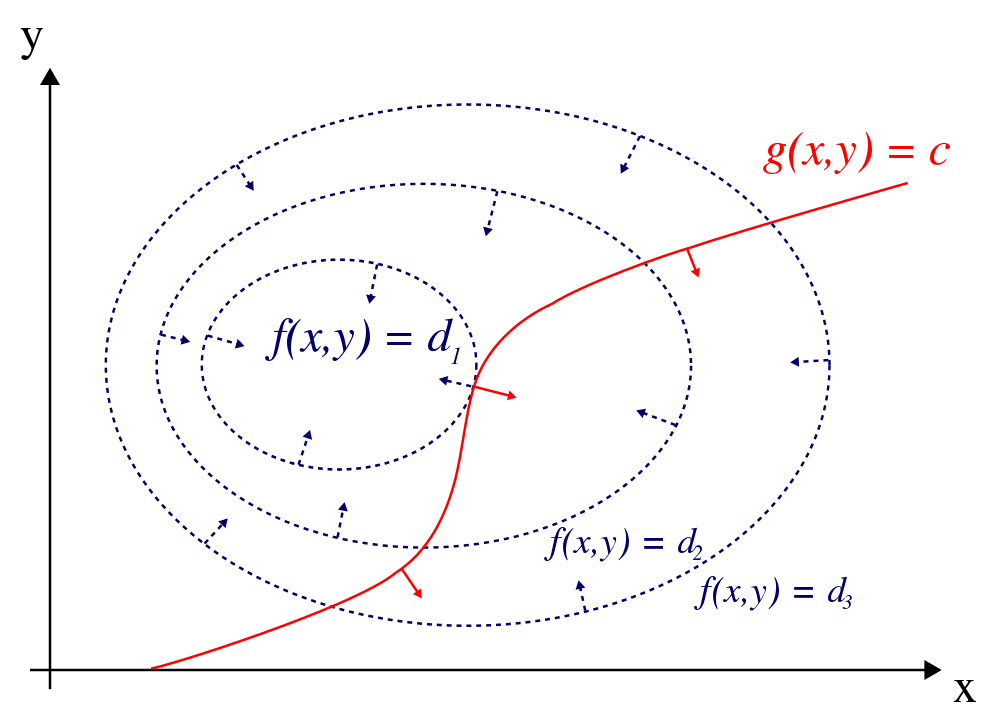
\includegraphics[width=1.05\linewidth]{figs/lagrange.png}
			\end{figure}
		\end{column}
	\end{columns}
\end{frame}


% -----------------------------------------------------------------------------

\begin{frame}[fragile, t]{(3) The advertisement problem}
	\begin{columns}
		\begin{column}{0.6\textwidth}
			\textbf{Introduction}\\ \vspace*{0.5em} 
			
			We want equal exposure to 4 segments.
			Given 2 advertisement channels and their associated reach in units of $\text{views} / \text{dollar}$, allocate the money.
			\begin{equation*}
				\begin{pmatrix}
				5\\ 
				4\\ 
				6\\ 
				3
				\end{pmatrix}
				x_1
				+
				\begin{pmatrix}
				2\\ 
				3\\ 
				7\\ 
				7
				\end{pmatrix}
				x_2
				=
				\begin{pmatrix}
				9 \\ 
				9\\ 
				9\\ 
				9
				\end{pmatrix}
				+
				\begin{pmatrix}
				e_1 \\ 
				e_2\\ 
				e_3\\ 
				e_4
				\end{pmatrix}
			\end{equation*}
			This problem can be formulated as
			\begin{align*}
			\text{minimize } \quad & \sum_{i=1}^{4} e_i^2 
			=  	\mathbf{e}^T \mathbf{e}	= \norm{ \mathbf{A} \mathbf{x} - \mathbf{b} }_2^2.
			\end{align*}
		\end{column}
		\begin{column}{0.4\textwidth}%
			\begin{center}
				\textbf{Views per unit of money}
			\end{center}
			\[
			A = 
			\begin{blockarray}{rcc}
			& \text{tv} & \text{paper}  \\
			\begin{block}{l(cc)}
			\text{y \female}  & 5 &  2 \\
			\text{y \mars}  & 4 &  3 \\
			\text{o \female}  & 6 &  7 \\
			\text{o \mars}  & 3 &  7 \\
			\end{block}
			\end{blockarray}
			\]
			\vspace*{-3em}
			\begin{figure}
				\centering
				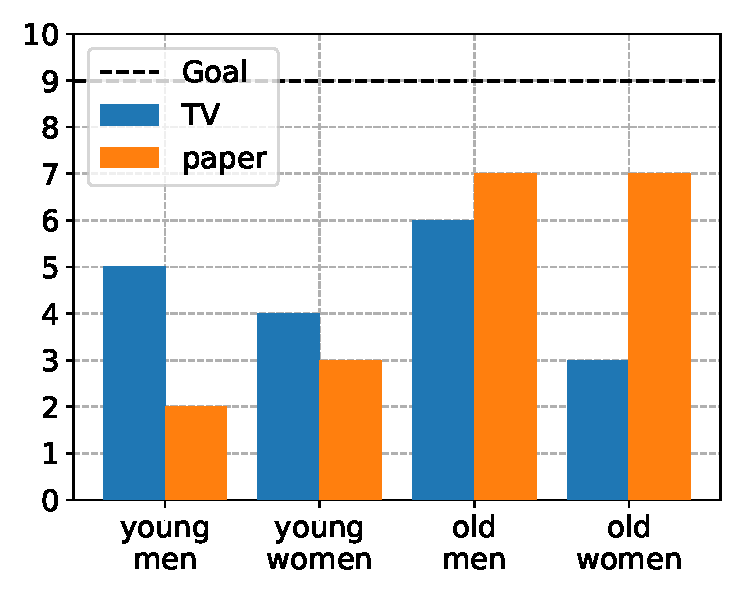
\includegraphics[width=1.0\linewidth]{figs/advertisement_statement.pdf}
			\end{figure}
		\end{column}
	\end{columns}
\end{frame}


\begin{frame}[fragile, t]{(3) The advertisement problem}
	\begin{columns}
		\begin{column}{0.5\textwidth}
			\textbf{Problem instance}
			\begin{align*}
			\text{minimize } \quad & 
			\mathbf{e}^T \mathbf{e}
			=
			\norm{ \mathbf{A} \mathbf{x} - \mathbf{b} }_2^2
			\end{align*}
			\textbf{Problem generalization}
			\\
			\vspace*{0.5em}
			Minimizing $\norm{ \mathbf{A} \mathbf{x} - \mathbf{b} }_2^2$ is a
			\emph{least squares problem}, solved analytically by the equation
			\begin{equation*}
				\mathbf{A}^T \mathbf{A} \mathbf{x} =\mathbf{A}^T \mathbf{b}.
			\end{equation*}
		\end{column}
		\begin{column}{0.5\textwidth}%
			\textbf{Solution}
			\begin{equation*}
			\begin{pmatrix}
			5\\ 
			4\\ 
			6\\ 
			3
			\end{pmatrix}
			\textcolor{titlered}{\mathbf{1.5}}
			+
			\begin{pmatrix}
			2\\ 
			3\\ 
			7\\ 
			7
			\end{pmatrix}
			\textcolor{titlered}{\mathbf{0.4}}
			=
			\begin{pmatrix}
			9 \\ 
			9\\ 
			9\\ 
			9
			\end{pmatrix}
			+
			\begin{pmatrix}
			-0.7 \\ 
			-1.8 \\ 
			\ \ 2.8 \\ 
			-1.7
			\end{pmatrix}
			\end{equation*}
			\vspace*{-1.8em}
			\begin{figure}
				\centering
				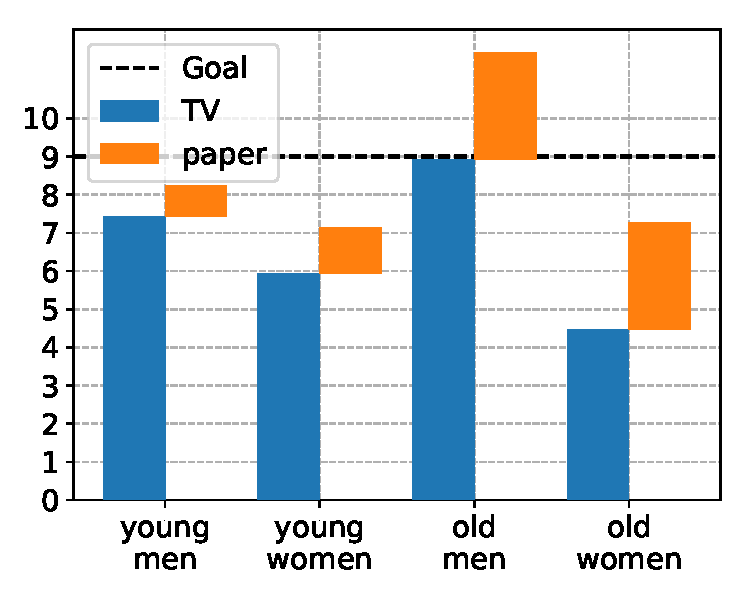
\includegraphics[width=0.8\linewidth]{figs/advertisement_statement_sol.pdf}
			\end{figure}
		\end{column}
	\end{columns}
\end{frame}


% -----------------------------------------------------------------------------

\begin{frame}[fragile, t]{(4) The \emph{constrained} advertisement problem}
	\begin{columns}
		\begin{column}{0.6\textwidth}
			\textbf{Introduction}\\ \vspace*{0.5em} 
			Same as before, but constrained by a budget of $1$ unit of money.
			\begin{equation*}
			\begin{pmatrix}
			5\\ 
			4\\ 
			6\\ 
			3
			\end{pmatrix}
			x_1
			+
			\begin{pmatrix}
			2\\ 
			3\\ 
			7\\ 
			7
			\end{pmatrix}
			x_2
			=
			\begin{pmatrix}
			9 \\ 
			9\\ 
			9\\ 
			9
			\end{pmatrix}
			+
			\begin{pmatrix}
			e_1 \\ 
			e_2\\ 
			e_3\\ 
			e_4
			\end{pmatrix}
			\end{equation*}
			This problem can be formulated as
			\begin{align*}
			\text{minimize } \quad & \sum_{i=1}^{4} e_i^2 = 
			\mathbf{e}^T \mathbf{e}
			=
			\norm{ \mathbf{A} \mathbf{x} - \mathbf{b} }_2^2 \\
			\text{subject to } \quad & x_1 + x_2 = 1 
			\end{align*}
		\end{column}
		\begin{column}{0.4\textwidth}%
			\begin{center}
				\textbf{Views per unit of money}
			\end{center}
			\[
			A = 
			\begin{blockarray}{rcc}
			& \text{tv} & \text{paper}  \\
			\begin{block}{l(cc)}
			\text{y \female}  & 5 &  2 \\
			\text{y \mars}  & 4 &  3 \\
			\text{o \female}  & 6 &  7 \\
			\text{o \mars}  & 3 &  7 \\
			\end{block}
			\end{blockarray}
			\]
			\vspace*{-3em}
			\begin{figure}
				\centering
				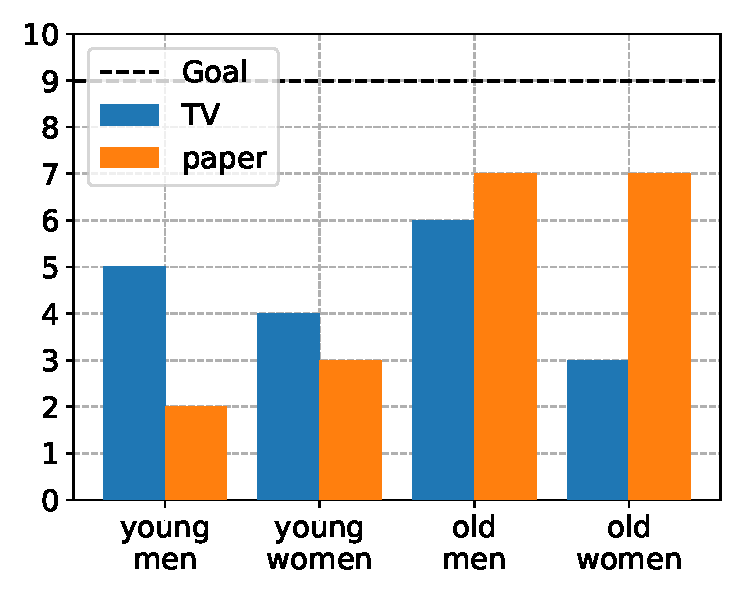
\includegraphics[width=1.0\linewidth]{figs/advertisement_statement.pdf}
			\end{figure}
		\end{column}
	\end{columns}
\end{frame}


\begin{frame}[fragile, t]{(4) The \emph{constrained} advertisement problem}
	\begin{columns}
		\begin{column}{0.5\textwidth}
			\textbf{Problem instance}
			\begin{align*}
			\text{minimize } \quad & 
			\mathbf{e}^T \mathbf{e}
			=
			\norm{ \mathbf{A} \mathbf{x} - \mathbf{b} }_2^2 \\
			\text{subject to } \quad & \mathbf{x}^T \mathbf{1} = 1
			\end{align*}
			\textbf{Problem generalization}
			\\
			\vspace*{0.5em}
			\emph{Constrained least squares problem}, solved by Lagrange multipliers and linear algebra.
			% the method of Lagrange multipliers and a set of KKT-equations.
			% Equation 16.4 in http://vmls-book.stanford.edu/vmls.pdf
			\begin{equation*}
			\begin{pmatrix}
			2\mathbf{A}^T \mathbf{A} & \mathbf{1} \\ 
			\mathbf{1} & 0
			\end{pmatrix}
			\begin{pmatrix}
			\hat{\mathbf{x}} \\ 
			\hat{\mathbf{z}}
			\end{pmatrix} 
			=
			\begin{pmatrix}
			2\mathbf{A}^T\mathbf{b}
			\\
			\mathbf{d}
			\end{pmatrix}
			\end{equation*}
		\end{column}
		\begin{column}{0.5\textwidth}%
			\textbf{Solution}
			\begin{equation*}
			\begin{pmatrix}
			5\\ 
			4\\ 
			6\\ 
			3
			\end{pmatrix}
			\textcolor{titlered}{\mathbf{0.6}}
			+
			\begin{pmatrix}
			2\\ 
			3\\ 
			7\\ 
			7
			\end{pmatrix}
			\textcolor{titlered}{\mathbf{0.4}}
			=
			\begin{pmatrix}
			9 \\ 
			9\\ 
			9\\ 
			9
			\end{pmatrix}
			+
			\begin{pmatrix}
			-5.1 \\ 
			-5.4 \\ 
			-2.6 \\ 
			-4.5
			\end{pmatrix}
			\end{equation*}
			
			\vspace*{-1.8em}
			\begin{figure}
				\centering
				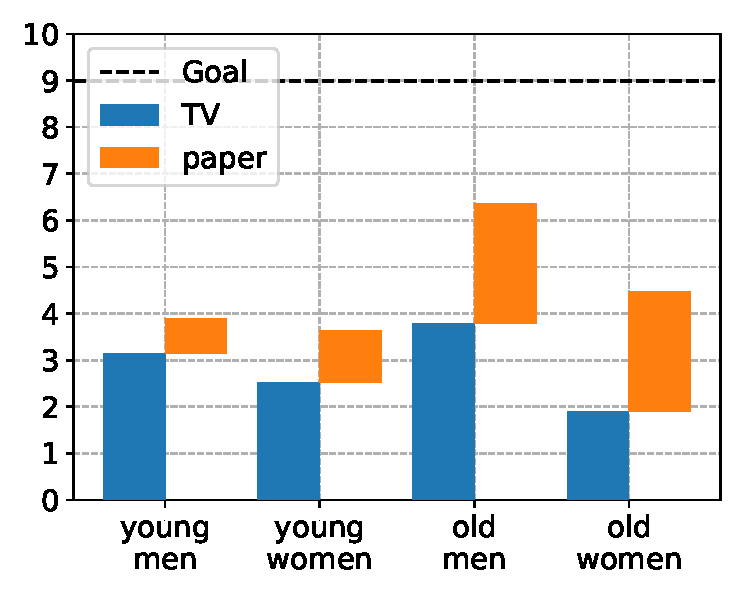
\includegraphics[width=0.8\linewidth]{figs/advertisement_statement_constr_sol.pdf}
			\end{figure}
		\end{column}
	\end{columns}
\end{frame}


% -----------------------------------------------------------------------------

\begin{frame}[fragile, t]{(5) The worker-assignment problem}
	\begin{columns}
		\begin{column}{0.6\textwidth}
			\textbf{Introduction}\\ \vspace*{0.5em} 
			Assign 4 workers to 4 tasks, given a matrix $C$ specifying to which degree workers enjoy each task.
			\\
			\vspace*{0.5em} 
			This amounts to specifying
			$X$ with entries in $X_{ij} \in \{0, 1\}$, i.e.
			\begin{equation*}
				X = \begin{pmatrix}
				0 & 1 & 0 & 0\\ 
				1 & 0 & 0 & 0\\ 
				0 & 0 & 0 & 1 \\ 
				0 & 0 & 1 & 0
				\end{pmatrix},
			\end{equation*}
			The above yields a satisfaction of
			\begin{equation*}
				6 + 4 + 8 + 1 = 19.
			\end{equation*}
			
			
		\end{column}
		\begin{column}{0.4\textwidth}%
			\textbf{Problem data}
			\[
			C = 
			\begin{blockarray}{rcccc}
			& A & B & C & D  \\
			\begin{block}{l	(cccc)}
			\text{ole}  & 5 &  6 & 1 &  6 \\
			\text{åse}  & 4 &  5 & 0 &  1 \\
			\text{dag}  & 1 &  2 & 6 &  8 \\
			\text{lise} & 7 &  2 & 1 &  1 \\
			\end{block}
			\end{blockarray}
			\]
			\textbf{Solution space growth}
			\begin{tabular}{rr}
				\toprule 
				$n$ & digits in $n!$  \\ \midrule
				$1$ & $1$ \\
				$10$ & $7$   \\
				$25$ & $26$   \\
				$50$ & $65$ \\ \bottomrule
			\end{tabular}
		\end{column}
	\end{columns}
\end{frame}


\begin{frame}[fragile, t]{(5) The worker-assignment problem}
	\begin{columns}
		\begin{column}{0.55\textwidth}
			\textbf{Problem instance}
			\begin{align*}
			\text{minimize } \quad & - \sum_i \sum_j C_{ij} X_{ij}  \\
			\text{subject to } \quad & \sum_i X_{ij} = 1 \text{ for every } j \\
			 & \sum_j X_{ij} = 1 \text{ for every } i
			\end{align*}
			\textbf{Problem generalization}
			\\
			\vspace*{0.5em}
			This is the \emph{assignment problem}, solved in $\mathcal{O}(n^3)$ time, not $\mathcal{O}(n!)$.
		\end{column}
		\begin{column}{0.45\textwidth}%
			\textbf{Solution}
			\[
			C_{ij} \widehat{X}_{ij} = 
			\begin{blockarray}{rcccc}
			& A & B & C & D  \\
			\begin{block}{l(cccc)}
			\text{ole}  & 5 &  6 & 1 &  \textcolor{titlered}{\mathbf{6}} \\
			\text{åse}  & 4 &  \textcolor{titlered}{\mathbf{5}} & 0 &  1 \\
			\text{dag}  & 1 &  2 & \textcolor{titlered}{\mathbf{6}} &  8 \\
			\text{lise} & \textcolor{titlered}{\mathbf{7}} &  2 & 1 &  1 \\
			\end{block}
			\end{blockarray}
			\]
			\begin{equation*}
				- \sum_i \sum_j C_{ij} \widehat{X}_{ij}
				=6 + 4 + 6 + 7 = 23
			\end{equation*}
		\end{column}
	\end{columns}
\end{frame}


% -----------------------------------------------------------------------------

\begin{frame}[fragile, t]{(6) The diet problem}
	\begin{columns}
		\begin{column}{0.475\textwidth}
			\textbf{Introduction}\\ \vspace*{0.5em} 
			Minimize the total cost of the diet, subject to the dietary constraints.
			
			{\small 
			\begin{alignat*}{3}
			\text{minimize } \quad & p_1 x_1 + p_2 x_2 + p_3 x_3 && \\
			\text{subject to } \quad & 16 x_1 + 5 x_2 + 12 x_3 && \geq 100 \\ % Synes egentlig x1, x2 og x3 skulle vært aligned nedover
			\quad & 150 x_1 + 100 x_2 + 40 x_3 && \geq 2000 \\
			\quad & 150 x_1 + 100 x_2 + 40 x_3 && \leq 2500
			\end{alignat*}
		
		``Minimize cost, but get 100 grams of protein, and between 2000 and 2500 calories.''
	}
			
			
		\end{column}
		\begin{column}{0.525\textwidth}%
			\textbf{Problem data}
			\small
			\begin{center}
				\begin{tabular}{llrr}
					\toprule 
					Food & Price & Protein & Calories \\ \midrule
					$x_1$  eggs & $p_1$ & 16 & 150 \\
					$x_2$ bread & $p_2$ & 5 & 100 \\
					$x_3$ milk & $p_3$ & 12 & 40 \\ \bottomrule
				\end{tabular}
			\end{center}
			{\tiny The numbers above are fictitious.}
			\normalsize
				\vspace*{0em}
				\begin{figure}
					\centering
					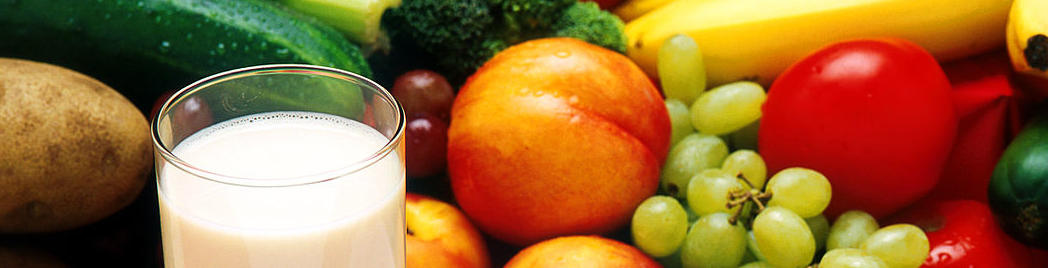
\includegraphics[width=1\linewidth]{figs/foods.jpg}
				\end{figure}
		\end{column}
	\end{columns}
\end{frame}


\begin{frame}[fragile, t]{(6) The diet problem}
	\begin{columns}
		\begin{column}{0.999\textwidth}
			\textbf{Problem instance}
			\small
			\begin{align*}
			\text{minimize } \quad & 
			\begin{pmatrix}
			p_1 & p_2 & p_3 
			\end{pmatrix}
			 \begin{pmatrix}
			 x_1 & x_2 & x_3 
			 \end{pmatrix}^{T}  \\
			\text{subject to } \quad & \begin{pmatrix}
			16 & 5 & 12 \\ 
			150 & 100 & 40\\ 
			-150 & -100 & -40
			\end{pmatrix}
			\begin{pmatrix}
			x_1  \\ 
			x_2 \\ 
			x_3
			\end{pmatrix}
			\geq 
			\begin{pmatrix}
			100  \\ 
			2000 \\ 
			-2500
			\end{pmatrix} \\
			\quad & x_1, x_2, x_3 \geq 0
			\end{align*}
			\normalsize
			\textbf{Problem generalization}
			\\
			\vspace*{0.5em}
			This is a \emph{linear program}. 
			Efficient algorithms exist.
			\begin{align*}
			\text{minimize } \quad & \mathbf{p}^T \mathbf{x}  \\
			\text{subject to } \quad & \mathbf{A} \mathbf{x} \geq \mathbf{b} \\
			\quad & \mathbf{x} \geq \mathbf{0}
			\end{align*}
			
		\end{column}
	\end{columns}
\end{frame}

% -----------------------------------------------------------------------------

\begin{frame}[fragile, t]{(7) The hotel problem}
	% problem 6.2, page  177 in Dasgupta
	\begin{columns}
		\begin{column}{0.475\textwidth}
		\textbf{Introduction}\\ \vspace*{0.5em} 
		
		We wish to travel 100 units of distance.
		There are many hotels along the way.
		Pick hotels to travel \textasciitilde10 units per day.
		\end{column}
		\begin{column}{0.525\textwidth}%
			
	\textbf{Problem instance} \\ \vspace*{0.5em} 
	Set $M = 10$. Find a sequence $h_1, h_2, \ldots, h_n$ to 
	\begin{align*}
	\text{minimize } \quad & 
	\sum_{j} \left(M - (h_{j} - h_{j-1})  \right)^2.
	\end{align*}

		\end{column}
	\end{columns}
	
	\begin{figure}
		\centering
		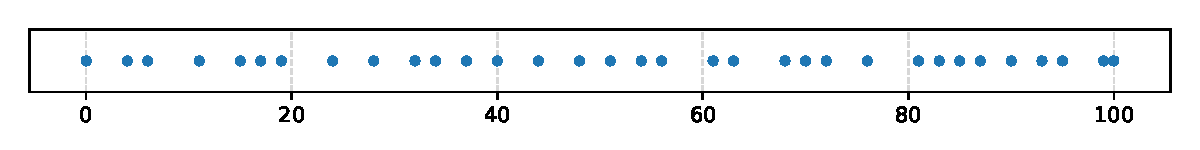
\includegraphics[width=1\linewidth]{figs/hotel_problem_instance_large.pdf}
	\end{figure}
	\vspace*{-1.5em}
	\textbf{Examples} \\ \vspace*{0.5em} 
	Traveling from $x = 0$ to $x = 6$ incurs a penalty of $(10 - (6 - 0))^2 = 4^2$. \\
	Traveling from $x = 0$ to $x = 11$ incurs a penalty of $(10 - (11 - 0))^2 = 1^2$.
	There are 31 hotels above, and $2^{31} = 2\,147\,483\,648$ possibilities.
	
\end{frame}


\begin{frame}[fragile, t]{(7) The hotel problem}
	\begin{columns}
		\begin{column}{0.5\textwidth}
			\textbf{Problem} \\ 
			Let $P(j)$ be the minimal penalty at stop $j$.
			Realize that
			\begin{align*}
			P(j) = \min_{ 0 \leq i < j}
			\left( P(i) + (M - (h_j - h_i))^2 \right).
			\end{align*}
			
			Solved in $\mathcal{O}(n^2)$ time, not $\mathcal{O}(2^n)$.
			
		\end{column}
		\begin{column}{0.5\textwidth}%
			\textbf{Problem generalization} \\ \vspace*{0.5em} 
			The solution technique is called \emph{dynamic programming} (DP).
			To use DP, we must (1) identify a recursive relationship, (2) define initial conditions and (3) solve problems in correct order.
		\end{column}
	\end{columns}
	
		\begin{figure}
			\centering
			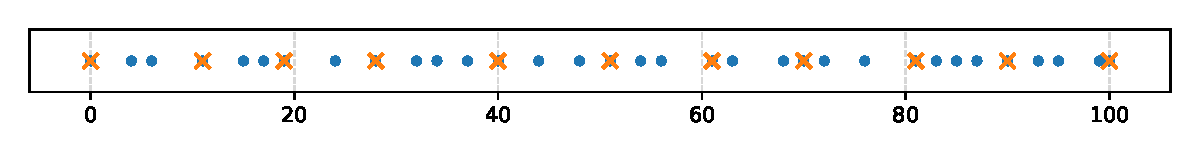
\includegraphics[width=1\linewidth]{figs/hotel_problem_instance_large_solution.pdf}
		\end{figure}
\end{frame}


% -----------------------------------------------------------------------------

\begin{frame}[fragile, t]{(8) The magnet problem}
	\begin{columns}
		\begin{column}{0.6\textwidth}
			\textbf{Introduction}\\ \vspace*{0.5em} 
			We are given $6$ magnets.
			Choose $x_i \in \{-1, 1\}$
			to minimize the total energy
			\begin{equation*}
				E(\mathbf{x}) = w_{12} x_1 x_2 + w_{13} x_1 x_3 + \cdots + w_{56} x_5 x_6.
			\end{equation*}
			The problem can be formulated as
			\begin{align*}
			\text{minimize } \quad & E(\mathbf{x}) = \mathbf{x}^T \mathbf{W} \mathbf{x}  \\
			\text{subject to } \quad & x_i \in \{-1, 1\}  .
			\end{align*}
			
			There are $2^{6-1}$ states, and $E(\mathbf{x})$ is not differentiable.
			A difficult problem.
		\end{column}
		\begin{column}{0.4\textwidth}%
			\textbf{Problem}\\
			\begin{figure}
				\centering
				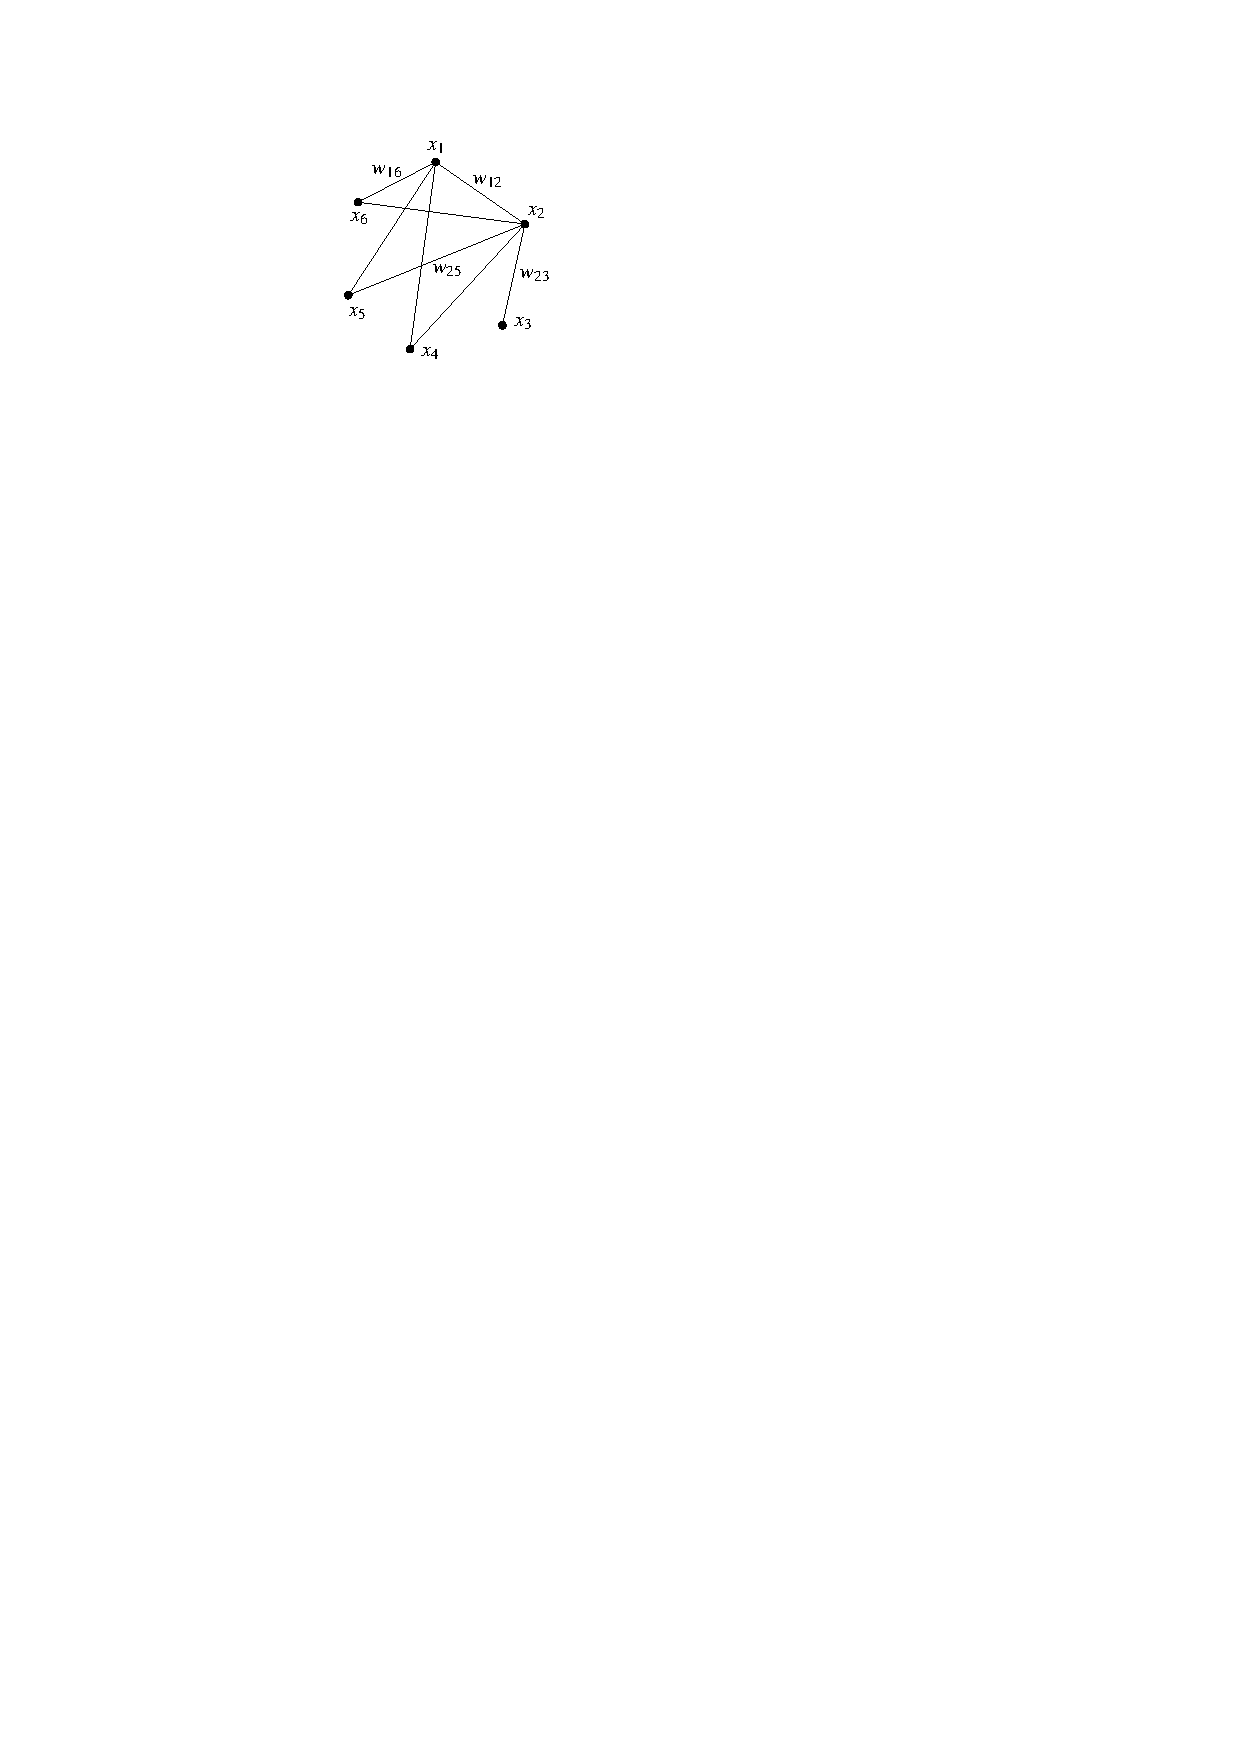
\includegraphics[width=0.8\linewidth]{figs/magnet_problem.pdf}
			\end{figure}
		\end{column}
	\end{columns}
\end{frame}


\begin{frame}[fragile, t]{(8) The magnet problem}
	\begin{columns}
		\begin{column}{0.55\textwidth}
			\textbf{Problem instance}
			\begin{align*}
			\text{minimize } \quad & E(\mathbf{x}) = \mathbf{x}^T \mathbf{W} \mathbf{x}  \\
			\text{subject to } \quad & x_i \in \{-1, 1\}  .
			\end{align*}
			\textbf{Problem generalization}
			\\
			\vspace*{0.5em} 
			\emph{Simulated annealing} balances exploitation and exploration. \\
			Widely applicable meta-heuristic.
			%When we have a (1) non-differentiable function with (2) a vast search space and (3) a notion of neighborhoods, use \emph{simulated annealing} to balance exploitation and exploration.
		\end{column}
		\begin{column}{0.45\textwidth}%
	\begin{figure}
		\centering
		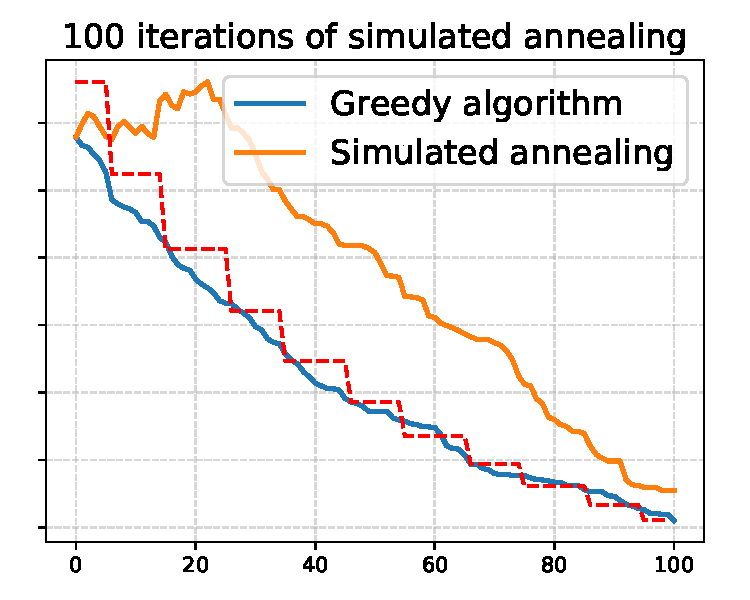
\includegraphics[width=1.1\linewidth]{figs/simulated_annealing.pdf} % What is the red dotted line?
	\end{figure}
		\end{column}
	\end{columns}
\end{frame}

% -----------------------------------------------------------------------------

\begin{frame}[fragile, t]{(9) The egg boiling problem}
	% https://www.youtube.com/watch?v=a79klpzaPgY
	% https://arxiv.org/pdf/1807.02811.pdf
	
	\begin{columns}
		\begin{column}{0.6\textwidth}
			\textbf{Introduction}\\ \vspace*{0.5em} 
			Let $b$ be the boiling time of an egg, $c$ be the cooling time, and $s$ be the amount of salt used.
			Let $f(b, c, s): \mathbb{R}^3 \to \mathbb{R}$ be the quality of a boiled egg.
			\\
			\vspace*{1em}
			This problem can be formulated as
			\begin{align*}
			\text{minimize } \quad & - f(b, c, s)  \\
			\text{subject to } \quad & b, c, s \geq 0 
			\end{align*}
			Evaluating $f(b, c, s)$ is expensive.
		\end{column}
		\begin{column}{0.4\textwidth}%
			\begin{figure}
				\centering
				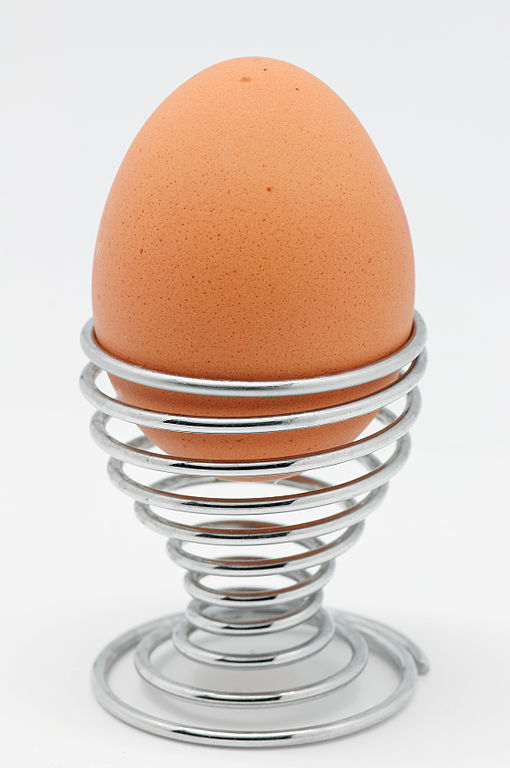
\includegraphics[width=0.8\linewidth]{figs/egg}
			\end{figure}
		\end{column}
	\end{columns}
\end{frame}


\begin{frame}[fragile, t]{(9) The egg boiling problem}
	% https://dash.harvard.edu/bitstream/handle/1/27769882/BayesOptLoop.pdf?sequence=1&isAllowed=y
	\begin{columns}
		\begin{column}{0.55\textwidth}
			\textbf{Problem generalization}
			\\
			\vspace*{0.5em} 
			Given a smooth function $f: \mathbb{R}^n \to \mathbb{R}$ which is expensive to evaluate.
			\begin{align*}
			\text{minimize } \quad & f(\mathbf{x}) \\
			\text{subject to } \quad & \mathbf{a} \leq \mathbf{x} \leq \mathbf{b} 
			\end{align*}
			\vfill
			Clever sampling via \emph{bayesian optimization}, which builds a probability distribution over functions.
			Exploration vs. exploitation.
		\end{column}
		\begin{column}{0.45\textwidth}%
			\begin{figure}
				\centering
				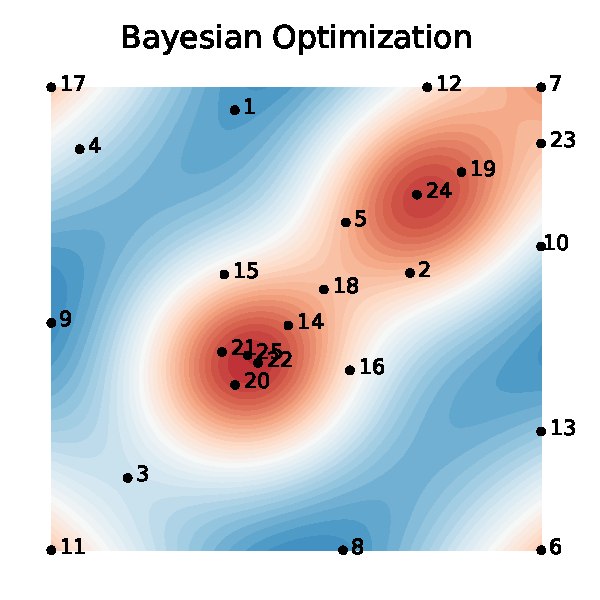
\includegraphics[width=1.05\linewidth]{figs/bayes_opt.pdf}
			\end{figure}
		\end{column}
	\end{columns}
\end{frame}

% -----------------------------------------------------------------------------

\begin{frame}[fragile, t]{(10) The brachistochrone problem}
	\textbf{Introduction}\\ \vspace*{0.5em} 
	
	A \emph{functional} is a function from a function to a real number.
	\begin{equation*}
		\text{functional} : \text{function} \to \text{real number}
	\end{equation*}
	\textbf{Problem} \\
	Find the path (i.e. function) minimizing the travel time of a bead.
	\begin{figure}
		\centering
		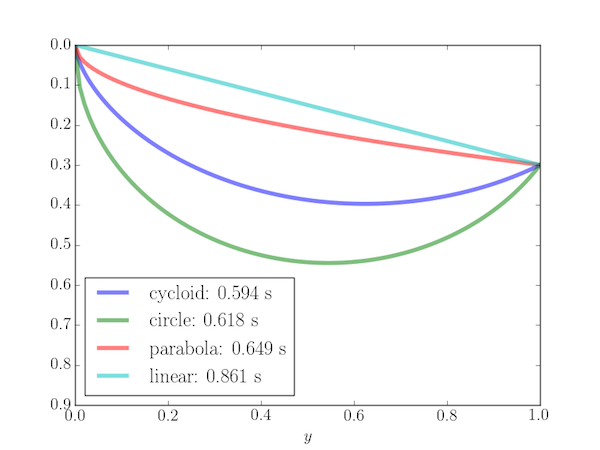
\includegraphics[width=0.5\linewidth]{figs/brachistochrone2.png}
	\end{figure}
\end{frame}


\begin{frame}[fragile, t]{(10) The brachistochrone problem}
	% https://www.youtube.com/watch?v=Cld0p3a43fU
	\begin{columns}
		\begin{column}{0.55\textwidth}
			\textbf{Problem generalization}
			\\ \vspace*{0.5em} 
			The problem amounts to minimizing a functional.
			In the space of all functions, find a function minimizing a functional.
			This is the domain of \emph{calculus of variations}.
			\vspace*{1em}
			
			Johann Bernoulli solved the problem in 1696.
			The solution is a cycloid.
		\end{column}
		\begin{column}{0.45\textwidth}%
			\begin{figure}
				\centering
				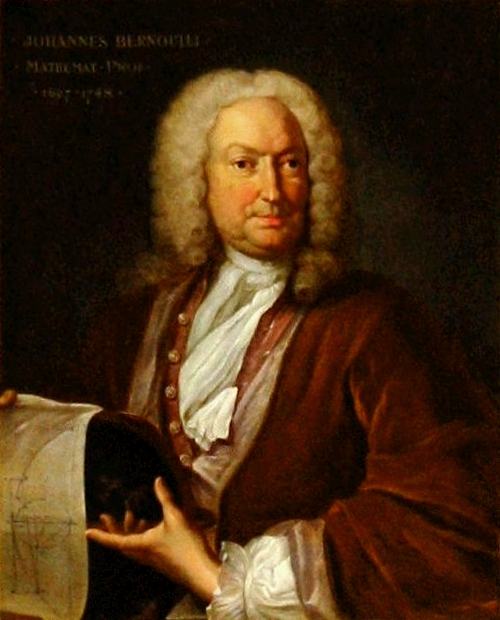
\includegraphics[width=0.8\linewidth]{figs/Johann_Bernoulli.jpg}
			\end{figure}
		\end{column}
	\end{columns}
\end{frame}


% -------------------------------------------------------------------------
\begin{frame}[fragile, t]{References (1/2)}
	\vspace{1em}
	\small
	\begin{easylist}[itemize]
		\ListProperties(Space=\listSpace, Space*=\listSpace)
		# Strang, Gilbert. \emph{Introduction to Applied Mathematics}. Wellesley, Mass: Wellesley-Cambridge Press, 1986.
		 
		## Chapter 3 -- ``The brachistochrone problem''
		## Chapter 7 -- ``The worker-assignement problem''
		## Chapter 8 -- ``The diet problem''
		
		# Boyd, Stephen, and Lieven Vandenberghe. \emph{Introduction to Applied Linear Algebra}. Cambridge University Press, 2018.
		 
		## Chapter 12 -- ``The advertisement problem''
		## Chapter 16 -- ``The constrained advertisement problem''
		
		# Dasgupta, Sanjoy, Christos H. Papadimitriou, and Umesh Virkumar. Vazirani. \emph{Algorithms}. Boston, Mass: McGraw Hill, 2008.
		
		## Chapter 6 -- ``The hotel problem''
	\end{easylist}
	\normalsize
\end{frame}

\begin{frame}[fragile, t]{References (2/2)}
	\vspace{1em}
	\small
	\begin{easylist}[itemize]
		\ListProperties(Space=\listSpace, Space*=\listSpace)
		# Duda, Richard O., Peter E. Hart, and David G. Stork. \emph{Pattern Classification}. 2 edition. New York: Wiley-Interscience, 2000.
		
		## Chapter 7 -- ``The magnet problem''
		
		# Jasper Snoek, Hugo Larochelle, Ryan P. Adams. \emph{Practical Bayesian Optimization of Machine Learning Algorithms}. arXiv.org, 2012.
		
		## ``The egg boiling problem''
	\end{easylist}
	\normalsize
	\vspace*{1em}
	\hrule
	
\begin{center}
	{\Large Thank you for your attention.} \\
	\vspace*{1em}
	Slides, \LaTeX{} source and Python code solving \\the problems and generating plots: \\
	\vspace*{1em}
	\url{github.com/tommyod/10_optimization_problems}
\end{center}
\end{frame}

\end{document}